\documentclass[11pt,a4paper]{article}


\setlength{\topmargin}{-55pt}%
\setlength{\oddsidemargin}{-20pt}%
\setlength{\textwidth}{490pt}%
\setlength{\textheight}{700pt}%
\setlength{\headsep}{20pt}%
\setlength{\headheight}{14pt}

\usepackage[utf8]{inputenc} % accents 8 bits dans le fichier
\usepackage[T1]{fontenc}      % accents codés dans la fonte
\usepackage[french]{babel}
\usepackage{amsmath,amssymb}
\usepackage{graphicx}
\usepackage{fancyhdr}
\usepackage{booktabs}
\usepackage{color, colortbl}
\usepackage{appendix}
\usepackage{pgfplots}
\usepackage[hidelinks]{hyperref}
\usepackage{siunitx}
\usepackage{algorithmicx}
\usepackage{algorithm}
\usepackage{algpseudocode}
\usepackage{subcaption}

\pgfplotsset{compat=1.3}

\addto\captionsfrench{% Replace "english" with the language you use
  \renewcommand{\contentsname}%
    {Table des matières}
}

\DecimalMathComma

\lhead{}      %en-tête
\chead{MPNA : Méthode des itérations simultanées}%
\rhead{}%
\lfoot{\tiny{Pierre GRANGER \& Matthias BEAUPERE}}
\cfoot{}%
\rfoot{\thepage}%
\renewcommand{\headrulewidth}{0.5pt}
\renewcommand{\footrulewidth}{0.5pt}
\pagestyle{fancy}

\newcommand{\HRule}{\rule{\linewidth}{0.5mm}}

\definecolor{green}{rgb}{0.2,0.8,0.2}

\begin{document}
\begin{center}

	{\LARGE\centering Projet de MPNA :\\ Méthode des itérations simultanées}\\[1cm]

	{ Matthias \bsc{Beaupère}, Pierre \bsc{Granger}}\\[0.5cm]
	{Rapport MPNA - CHPS - \today}
\end{center}

\tableofcontents

\section{Introduction et position du problème}
	De nombreux problèmes modernes impliquent le calcul de valeurs propres et de vecteurs propres de grandes matrices creuses. Par exemple, ce problème peut être rencontré lors de l'étude de certains systèmes physiques ou bien par exemple dans les moteurs de recherche qui reposent sur ce type de technique. Des algorithmes spécifiques doivent être utilisés afin de résoudre ces problèmes de valeur propre en un temps raisonnable. De plus les algorithmes utilisés doivent pouvoir être facilement utilisés sur les architectures massivement parallèles actuelles ce qui représente un grand défi.

\section{Approche utilisée}

\section{Cas séquentiel}

	\subsection{Description de l'algorithme général}

		Données du problèmes :

		\begin{itemize}
			\item $m$ : taille du sous-espace de Krylov
			\item $k$ : nombre de vecteurs propres demandé
			\item $p$ : précision demandé
			\item $A$ : matrice de taille $n*n$ donnée en entrée
			\item $N$ : nombre d'itérations
		\end{itemize}

		\begin{algorithm}
			\caption{Algorithme général}
			\begin{algorithmic}[1]
					\State $Q \gets rand()$
					\While {$i = 0 .. N-1$ OU max(precisions) < p}
						\State $Z = AQ$
						\State Gram-Schmidt $Q$
						\State Projection $B = Z^tAZ$
						\State Décomposition de Schur $B = Y^tRY$
						\State Retour dans l'espace d'origine $Q = ZY$
						\State Sélection des $k$ vecteur propres
						\State Calcul de la précision
					\EndWhile
				\end{algorithmic}
		\end{algorithm}

		Dans les paragraphes suivant sont détaillés chaque étape de l'algorithme.

		\subsubsection{Procédé de Gram-Schmidt}

			On utilise une décomposition QR avec le procédé de Gram-Schmidt pour orthonormalisé la matrice Q. L'ortogonalisation consiste chaque vecteur de la matrice $Z$ dans un vecteur temporaire tout en lui soustrayant son projeté sur chaque vecteur déjà ajouté. On normalise ensuite en divisant chaque vecteur par sa norme.

			\begin{algorithm}
				\caption{Algorithme de Gram-Schmidt}
				\begin{algorithmic}[1]
					\For {$i = 0..m-1$}
						\State $q^{temp}_i \gets q_i$
						\For{$k = 0..i$}
						\State $q^{temp}_i \gets q^{temp}_i - q_k(q_k.q_i)$
						\EndFor
					\EndFor
					\State $Q \gets Q^{temp}$
				\end{algorithmic}
			\end{algorithm}

		\subsubsection{Décomposition de Schur}

		La décomposition de Schur permet de calculer les valeurs et vecteurs propre de l'espace de Krylov, aussi appelés valeurs et vecteurs de Ritz. Pour ce calcul a été utilisé la bibliothèque \texttt{lapacke}.

		\subsubsection{Sélection de $k$ vecteurs propres}

			En entrée du programme est précisé le nombre $k$ de vecteurs propres désirés. La précision est calculé uniquement sur les $k$ vecteurs de plus grande valeur propre associée. Pour sélectionner ces vecteur, on range les vecteurs par valeur propre associée puis on ne garde que les $k$ premiers.

		\subsubsection{Calcul de la précision}

	\subsection{Étude de performances théorique}
		
		\subsubsection{Objectif en précision ou en itération}
			
			La terminaison du programme est donnée par deux critères suivant les paramètres entrée par l'utilisateur :
			\begin{itemize}
				\item Un objectif en précision : pour un exposant $p$ donné en argument, le programme termine si les $k$ vecteurs propres ont une précision inférieure à $10^{-p}$.
				\item Un objectif en itération : pour un entier $i$ donné en entrée, le programme termine si on atteint l'itération $i$.
			\end{itemize}

			Pour les formules de complexité, on supposera que l'objectif est de $N_{iter}$ itérations, même si en pratique le calcul s'arrête dans le cas où l'objectif en précision est spécifié et atteint avant l'objectif en itération.

		\subsubsection{}


			$$
			C^{tot} = N_{iter} * (C^{mm} + C^{GM} + C^{Proj} + C^{Schur} + C^{mm} + C^{select} + C^{préci})
			$$

			\paragraph{Produit de matrices :} $C^{mm} = O(N^2)$


	\subsection{Étude de performances pratique}



	\subsection{Ajout d'une méthode de déflation "Locking"}
		Toutes les valeurs propres de la matrice possèdent une vitesse de convergence différente par la méthode des itérations simultanées. Cela nous amène à affiner et recalculer constamment des vecteurs déjà connus avec la bonne précision ce qui entraine une perte de temps de calcul. De plus, des vecteurs propres qui ont déjà convergés jusqu'à la bonne précision peuvent perdre en précision à cause d'instabilités numériques au fil des calculs : la précision de certains vecteurs propres peut osciler au cours des itérations.

		Afin de résoudre ces deux problèmes nous avons décidé de mettre en place une méthode de déflation appelée "locking". Le principe est simple : lorsqu'un vecteur propre a convergé jusqu'à la précision désirée, on le verrouille de sorte à ne plus le remultiplier par la matrice $A$ et on diminue la taille du sous-espace de Krylov d'une unité. Néanmoins, on utilise toujours ce vecteur pour l'orthonormalisation afin qu'il guide la convergence correcte des veteurs restants.

	\subsection{Conclusions}

\section{Cas parallèle}
	
	\subsection{Approche utilisée}
	\subsection{Étude de performances théorique}
	\subsection{Étude de performances pratique}
	\subsection{Conclusions}

\section{Conclusion générale}

% FIGURES A AJOUTER
\begin{figure}
	\centering
	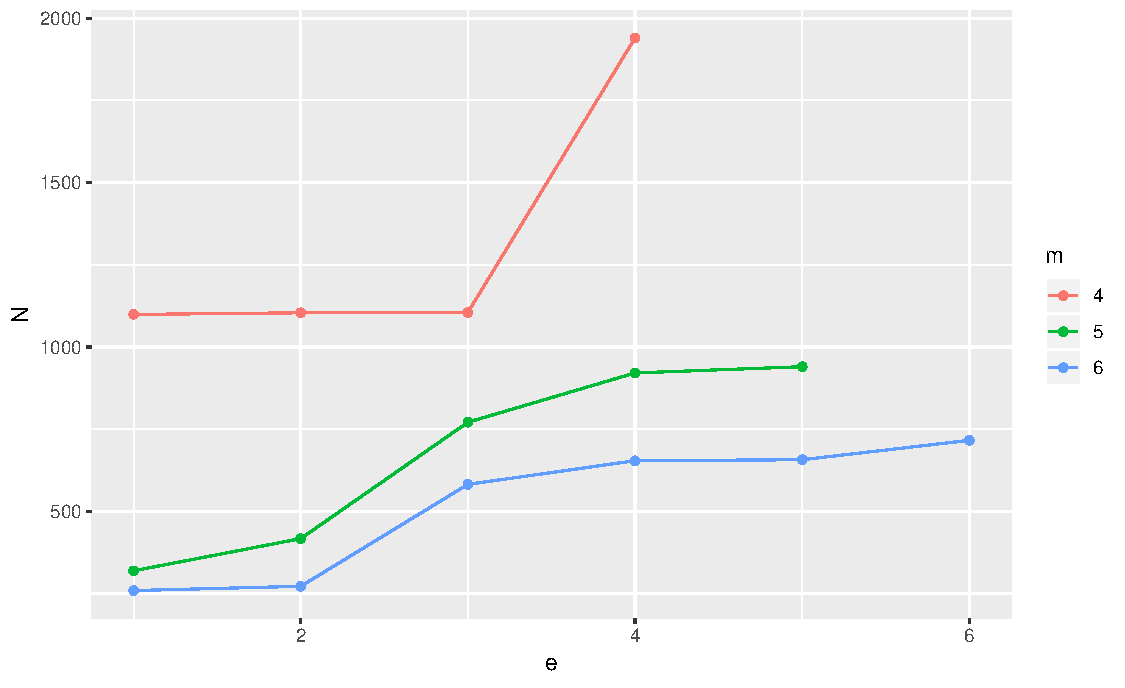
\includegraphics[width=0.8\linewidth, keepaspectratio]{plots/Nvse-m_p6.pdf}
	\caption{Nombre d'itérations $N$ nécessaires pour faire converger $e$ valeurs propres pour différentes tailles de sous-espace de Krylov $m$ et une précision $p=\SI{e-6}{}$ \label{fig:Nvse-m_p6}}
\end{figure}

\begin{figure}
	\centering
	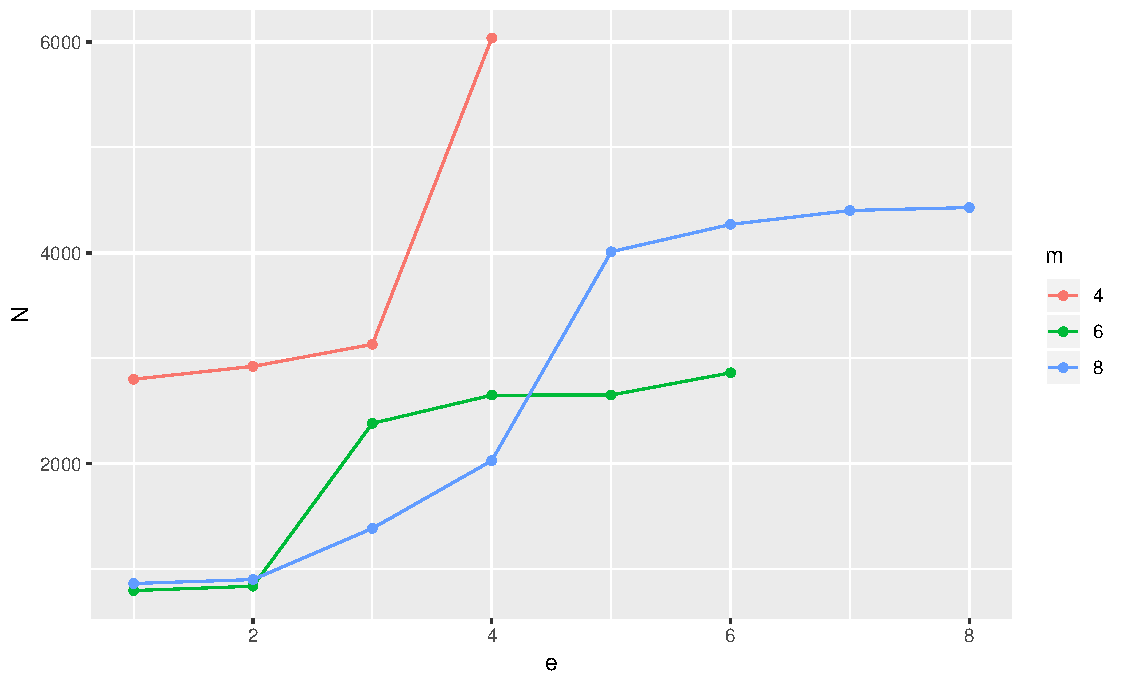
\includegraphics[width=0.8\linewidth, keepaspectratio]{plots/Nvse-m_p8.pdf}
	\caption{Nombre d'itérations $N$ nécessaires pour faire converger $e$ valeurs propres pour différentes tailles de sous-espace de Krylov $m$ et une précision $p=\SI{e-8}{}$ \label{fig:Nvse-m_p8}}
\end{figure}

\begin{figure}
	\centering
	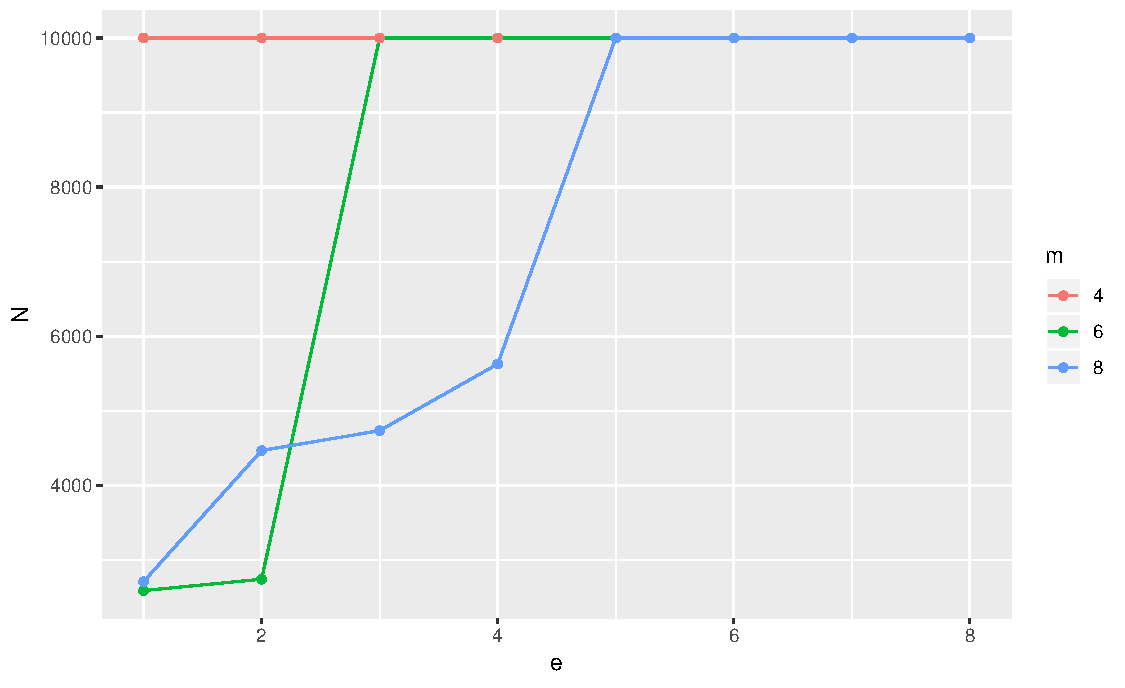
\includegraphics[width=0.8\linewidth, keepaspectratio]{plots/Nvse-m_p10.pdf}
	\caption{Nombre d'itérations $N$ nécessaires pour faire converger $e$ valeurs propres pour différentes tailles de sous-espace de Krylov $m$ et une précision $p=\SI{e-10}{}$ \label{fig:Nvse-m_p10}}
\end{figure}

\begin{figure}
	\centering
	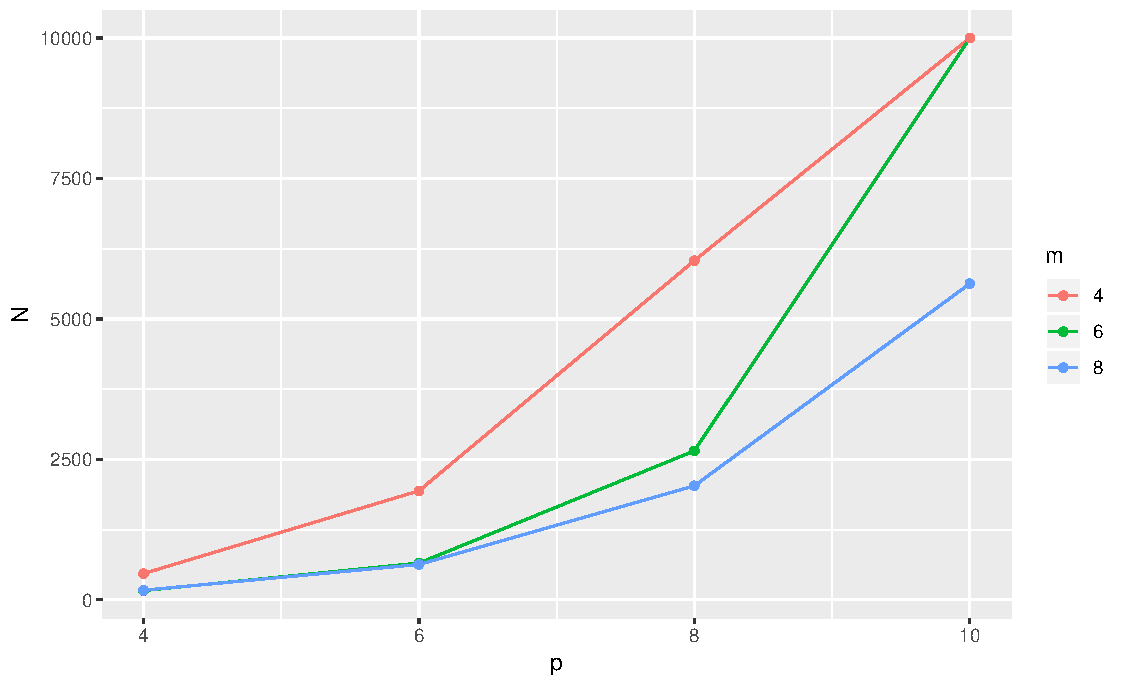
\includegraphics[width=0.8\linewidth, keepaspectratio]{plots/Nvsp-m_e4.pdf}
	\caption{Nombre d'itérations $N$ nécessaires pour faire converger $e = 4$ valeurs propres pour différentes tailles de sous-espace de Krylov $m$ et une précision $p$ \label{fig:Nvsp-m_e4}}
\end{figure}

\begin{figure}
	\centering
	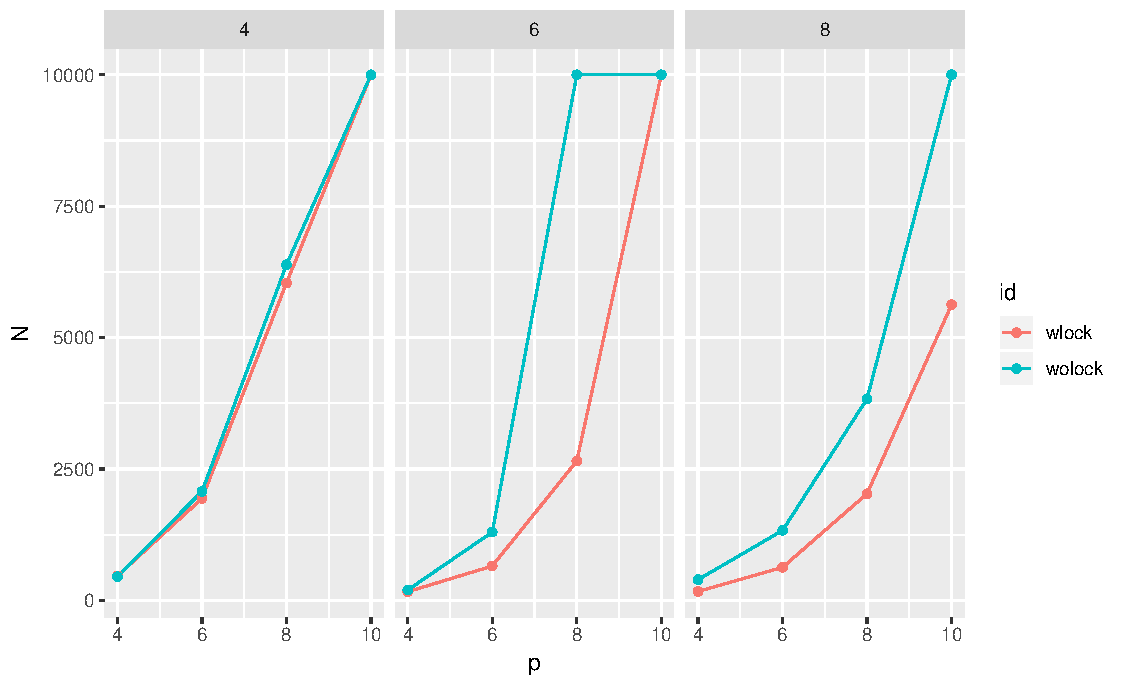
\includegraphics[width=0.8\linewidth, keepaspectratio]{plots/Nvsp_complock.pdf}
	\caption{Nombre d'itérations $N$ nécessaires pour faire converger $e = 4$ valeurs propres pour différentes tailles de sous-espace de Krylov $m$ et une précision $p$ avec et sans utilisation du locking \label{fig:Nvsp_complock}}
\end{figure}

\begin{figure}
	\centering
	\begin{subfigure}{0.49\linewidth}
		\centering
		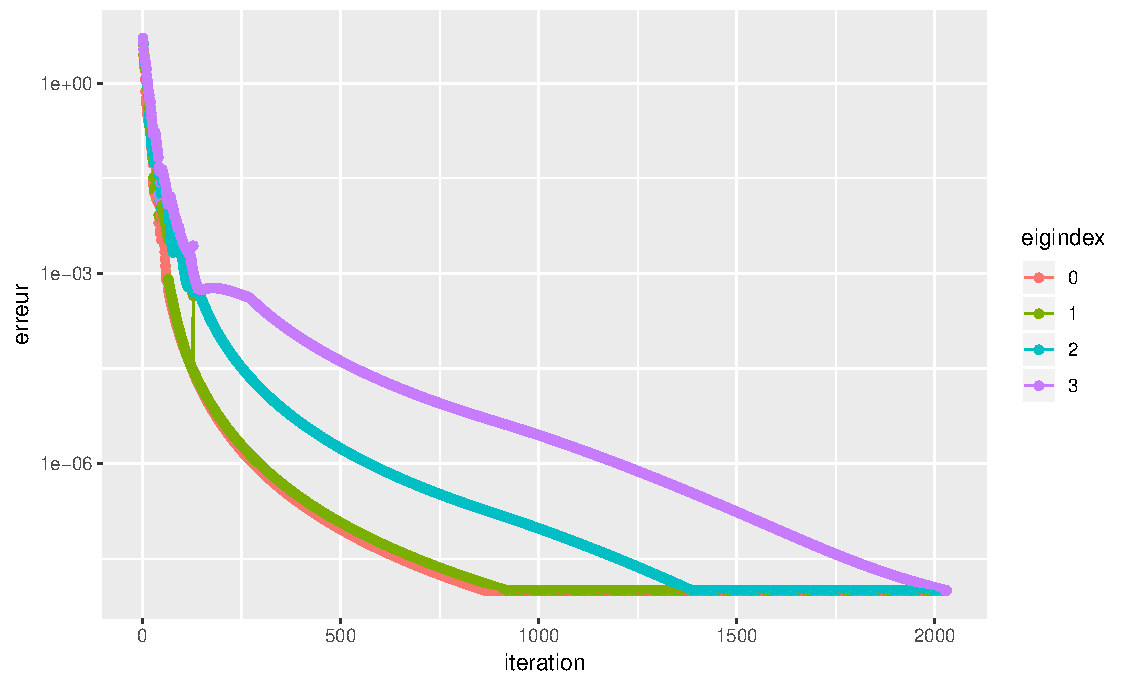
\includegraphics[width=\linewidth, keepaspectratio]{plots/wlock_e4_p8_m8.pdf}
		\caption{Avec locking\label{wlock_e4_p8_m8}}
	\end{subfigure}
	\begin{subfigure}{0.49\linewidth}
		\centering
		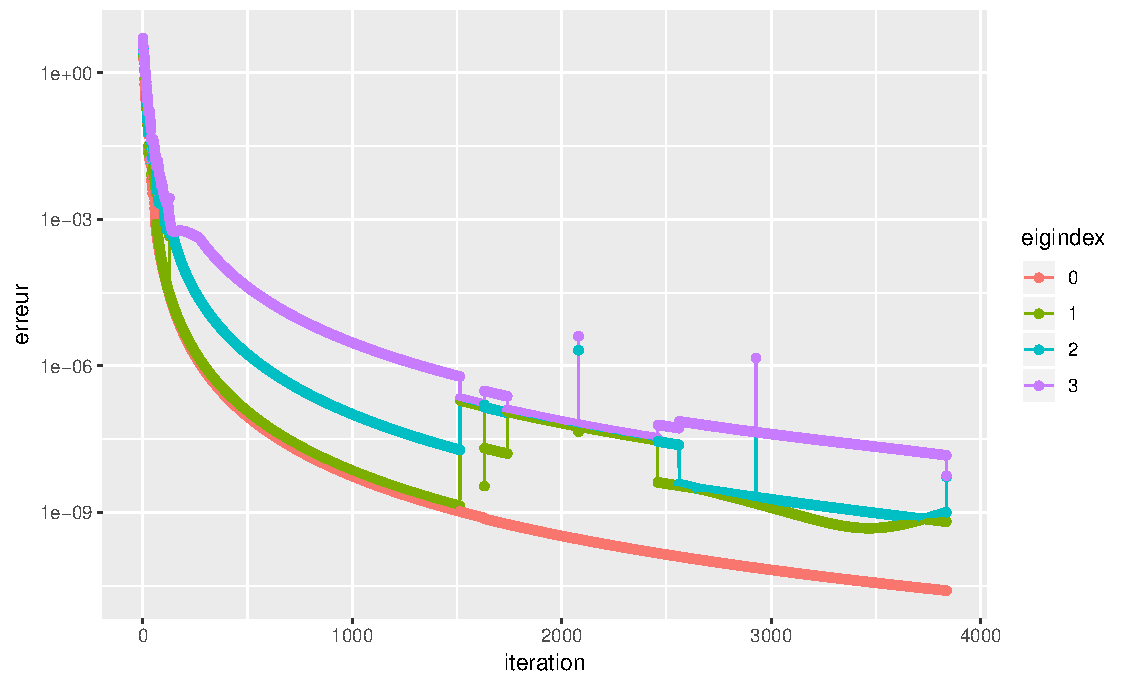
\includegraphics[width=\linewidth, keepaspectratio]{plots/wolock_e4_p8_m8.pdf}
		\caption{Sans locking\label{wolock_e4_p8_m8}}
	\end{subfigure}
	\caption{Précision au cours des itérations $N$ pour $e = 4$ valeurs propres pour une taille de sous-espace de Krylov $m=8$\label{fig:comp_locks}}
\end{figure}

On représente sur la figure \ref{fig:comp_locks} la précision au cours des itérations pour $e$ et $m$ fixés dans le cas de la méthode initiale et de la méthode avec locking. On peut tout d'abord observer que la convergence est bien plus rapide lorsque le locking est utilisé (environ 2000 contre 3800 itérations). On peut en outre constater sur la figure \ref{wlock_e4_p8_m8} que la convergence avec locking semble moins instable.


% \bibliographystyle{unsrt}
% \bibliography{synopsis.bib}

%\input{appendix}

\end{document}
